%++++++++++++++++++++++++++++++++++++++++
% Don't modify this section unless you know what you're doing!
\documentclass[a4paper,14pt]{article}
\usepackage{listings} % code blocks
\usepackage{tabularx} % extra features for tabular environment
\usepackage{amsmath}  % improve math presentation
\usepackage{graphicx} % takes care of graphic including machinery
\graphicspath{{figures/}}
\usepackage{subcaption} % necessary for subfigures
\usepackage[margin=2cm,a4paper,nohead]{geometry} % decreases margins
\usepackage{cite} % takes care of citations
\usepackage[final]{hyperref} % adds hyper links inside the generated pdf file

%++++++++++++++++++++++++++++++++++++++++


\begin{document}

\title{Exercise 3: Visual Planning with CNNs}
\author{Badhreesh M Rao, David-Elias K\"unstle}
\date{18/12/2017}
\pagenumbering{gobble} % turn of page numbering (not needed for 2 pages)
\maketitle
\section{Introduction}

The most famous use of convolutional neural networks (CNNs) is in image classification.
In contrast, here we describe their application for a planning task from visual input.
An agent has to find a target in a two dimensional maze  (\autoref{fig:maze}) from a random starting
position. The agent receives only partial observations (pob) of the environment.

\begin{figure}[h]
  \centering
  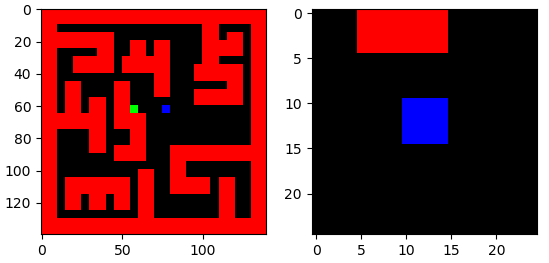
\includegraphics[width=0.7\textwidth]{maze}
  \caption{The agent (blue) has to find the target (green) in the maze (left,
    walls in red). It is only provided a history of partial observations
    (right).}
  \label{fig:maze}
\end{figure}

At each time step, the agent has to decide the direction (up, right, down, left)for the current timestep and some preceding pob.
Pob and optimal directions for training and validation are generated via
A-Star-Algorithm.
For testing, the agent has to maximize the number of successful runs.
A run is only successful if the agent finds the target in a limited amount of time.
In \autoref{sec:generalization}, we investigate the influence of changing target position, map,
history and pob on the test performance.

\section{Implementation}

Our agent is implemented via stacked convolution layers as described in
\autoref{tab:architecture} using the \emph{keras} library with \emph{tensorflow} backend.
The architecture resulted via trial and error.
As default we use the provided map in \autoref{fig:maze}, a history of 4 pob as input data
and a fixed target position.
We use the input history as a flat vector (1 channel) as provided.
Experiments with reshaping to two (width, height; history as channels) or three
(width, height, history; 1 channel) dimensions did not result in significant
better results.

\textbf{How well does the agent perform from the local view?}

Trained with Adam optimization (batch size $32$, learning rate $0.001$), we reached over $98\%$
accuracy on the validation set after 5 iterations over the full training data
(epochs).
In the test setup, the agent can usually find the target in less than 50 steps from any random start position. The agent seems to follow the shortest path directly to the target.

\begin{table}[h]
  \centering
  \begin{tabular}{ll}
    \hline
    Convolution Layer & (8 filters, size 64) \\
    Convolution Layer & (16 filters, size 32) \\
    Convolution Layer & (32 filters, size 16) \\
    Convolution Layer & (32 filters, size 8) \\
    Convolution Layer & (32 filters, size 4) \\
    Dense Layer & (5 outputs, softmax activation) \\
    \hline
  \end{tabular}
  \caption{Network architecture. A convolution layer here includes ReLu
    activation function and max pooling (size 2, stride 2).}
  \label{tab:architecture}
\end{table}

\textbf{ What happens if you increase the history length for the views or make the
view larger ?}

In the original layout, the history length was set to 4. With this and other parameters set up, the agent was able to find the target easily in the testing phase. With increasing values of history length, the training time slight increases and also the testing accuracy of the agent decreases.
This might be because if the agent is trained with a high history length, it remembers the start position and learns a path to the target.

In testing, if the agent does not appear in one of those starting positions, it will not be able to reach the target. It gets stuck in the starting stage.
In other words, the ability of the agent to generalize, or to reach its goal no matter where it appears on the map, decreases as the history length is increased.
If the view is made larger, then it becomes easier for the agent to reach its target. For the same history length, the agent with the larger view was able to reach its target more often than the agent with the smaller view. \autoref{fig:largerview} shows the map to the left and the larger view of the agent to the right (30x30 compared to 25x25 in \autoref{fig:maze}).

\begin{figure}[h]
  \centering
  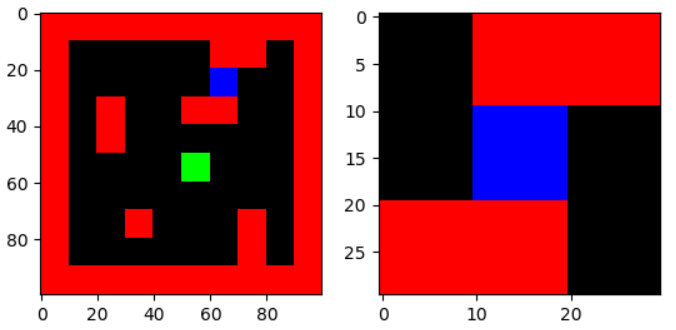
\includegraphics[width=0.7\textwidth]{larger_view}
  \caption{The agent (blue) now has a larger view and has to find the target (green) in the maze (left,
    walls in red). It is only provided a history of partial observations
    (right).}
  \label{fig:largerview}
\end{figure}

\section{Generalization}\label{sec:generalization}

Until this point the test situation was very close to the training situation.
Here we try, how our agent performs if the task (target position) or
environment (walls in maze) is changed after training.

\begin{figure}
    \centering
    \begin{subfigure}[b]{0.3\textwidth}
        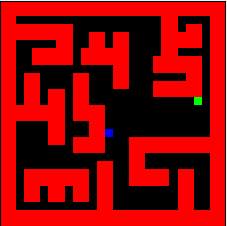
\includegraphics[width=\textwidth]{random_target}
        \caption{randomized target position}
        \label{fig:randomtarget}
    \end{subfigure}
    ~ %add desired spacing between images, e. g. ~, \quad, \qquad, \hfill etc.
      %(or a blank line to force the subfigure onto a new line)
    \begin{subfigure}[b]{0.3\textwidth}
        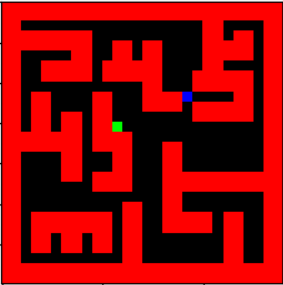
\includegraphics[width=\textwidth]{modified_map}
        \caption{slightly modified maze}
        \label{fig:modifiedmap}
    \end{subfigure}
    \caption{The agent tries using the way it learned while training to a fixed
      position where it expects the target. Once some pob history occurs, which the agent has
      not seen while training it is stuck by moving back and forth.}\label{fig:generalization}
\end{figure}

\subsection{Target location}

\textbf{What happens if you change the target location after training?}

If the target is at the fixed position, it looks like our agent magically knows
where it is and takes the shortest path.
This illusion is revealed, if the target is placed on any free, random position (\autoref{fig:randomtarget}).
The agent still moves straight to the middle of the map where the target was
while learning. As soon as the target should appear in the pob but doesn't, the
agent starts moving back and forth.
Therefore it usually doesn't reach any target while testing.

The target could also be placed such, that the agent has to pass it at the usual
path. Then the agent often also starts moving back and forth.
We could conclude, that it hasn't even learned to go to the target if it is
visible (target is in the current pob).

\subsection{Map}

\textbf{What happens if you change the map after training (how well does your agent generalize) ?}

If the map is changed after training (\autoref{fig:modifiedmap}), the agent does not generalize well to the new map layout in the testing phase, as it did with the map layout it was trained on.
Basically, if the agent comes across a new obstacle in the map which it did not see before during training, it will get stuck at that place, unable to proceed to its target. But if the agent appears in places where the new obstacle does not affect its path, the agent is able to reach its goal.

\subsection{Proposal}
\textbf{Can you think of ways to make the agent generalize across target locations in different maps ?}

A possible implementation of making the agent generalize across target locations in different maps would be to train the agent with training data obtained from different map and location configurations. Doing this would perhaps help the agent to generalize to situations where either the map layout or the target locations are different. 


% \begin{thebibliography}{99}
% \end{thebibliography}

\end{document}
